
In this section we describe CHARM, our proposed model for inferring personal attributes from conversations. As illustrated in Figure \ref{pipeline}, CHARM's operation consists of two stages: \emph{cue detection} and \emph{value ranking}. 
As input CHARM receives the user's utterances $U=u_0..u_N$ that contain a set of terms $t_0..t_M$, for example, $U=${\em 
\{``I stayed late at the \textbf{library} yesterday'', ``\textbf{Studied} for the \textbf{exam} so I could have better \textbf{grades} than my \textbf{classmates}''}\}. 
In the first stage, the term scoring model assigns a score to each term in the user's utterances, yielding $l_0..l_M$. The highest scoring terms are then selected to form a query $Q=q_0..q_K$, characterizing the user's correct attribute value, e.g., $Q=$``library studied exam grades classmates'' for the \emph{profession} attribute. 

In the second stage, $Q$ is evaluated against an external document collection $D=d_0..d_L$; each document in $D$ is associated with possible attribute values.  
Documents such as \emph{Wiki:Student} and \emph{Wiki:Dean's List}
\footnote{Wikipedia pages: \href{https://en.wikipedia.org/wiki/Student}{{Student}} \& \href{https://en.wikipedia.org/wiki/Dean\%27s_list}{{Dean's\_list}}}, which are associated with the attribute value \emph{student}, would score high with the example query.
The score aggregator then ranks the attribute values based on the documents' scores $s_0..s_L$, for instance, yielding a high attribute score for \emph{student} given our example utterances. The list of attribute values $V$ is \textbf{known} in advance (e.g., taken from Wikipedia list of professions); however, potentially only a subset of values $S \subset V$ have instances \textbf{seen} during training.


\begin{figure}[t!]
\centering
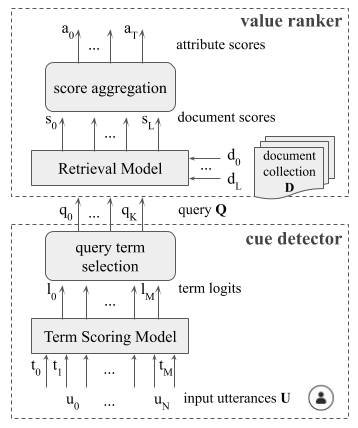
\includegraphics[width=0.45\textwidth]{imgs/scheme.png}
\vspace*{-0.3cm}
\caption{The pipeline of CHARM.
The Term Scoring Model assigns scores $l_0 .. l_M$ to the terms in the input utterances $u_0..u_N$. The terms with the highest scores are passed to the Retrieval Model, which queries the document collection $D$. The document scores are aggregated to produce attribute value scores
for predictions.
}
\label{pipeline}
\end{figure}

The rank of the correct attribute value acts as a distant supervision signal, allowing us to train term selection, regardless of the non-differentiable \texttt{argmax} operation.
CHARM is trained using reinforcement learning via the REINFORCE policy gradient method described in the previous section.


\subsection{Cue detection}
\label{sec:term-selection}

The  term scoring model $\delta$ evaluates how useful
each word in a given user's utterances is for making a prediction,
and assigns real-value scores $l_0 ... l_M$ to the terms accordingly. 
That is,
    $l_j = \delta (t_j | t_0, .. t_M; W)$,
where $W$ denotes the parameters of the model. The term scores $l_0 .. l_M$ are then used to select the words which will form the query for the value ranking component. 

Due to our use of REINFORCE, the selection process differs between the training and prediction settings.
During training, the scores $l_0 .. l_M$ are normalized with a softmax function to obtain
probabilities $p_0 ... p_M$, which are used to incrementally sample without replacement a query consisting of $K$ terms. The query length $K$ is a hyperparameter, optimized in the grid search.
The sampling in effect allows the words with low scores a better chance to be selected,
thus encouraging exploration. At inference time the query is formed by taking the terms with $K$ top scores.
%In our example, the word `library' will have a greater probability to be sampled during training time, %and 
%will only be selected during test time if its score is high enough to get into the top $K$ terms.

The term scoring model 
should produce high scores for terms that are descriptive of the user and of the attribute in general, instead of a specific attribute value. This means that it should be able to exploit background knowledge and a term's context to 
judge its relevance to the attribute.
For instance, having seen the phrase \emph{``stayed late at the hospital''} for the 
\emph{physician} at training time, at prediction time an ideal model would correctly estimate the importance of the word `\textit{library}' in the phrase \emph{``stayed late at the library''}, even if there were no instances of \emph{student} in the training set. Considering this, we give preference to the models that operate on sequences, as opposed to the bag-of-word models. We select BERT \cite{devlin2018bert} as our term scoring model, because it is a sequential model incorporating world knowledge that should effectively use word context, predicting whether terms are related to an attribute.

For further description, let us suppose the cue detector picks the words $Q = q_0 ... q_K$ as the query terms for CHARM's value ranking stage. A typical query would consist of the terms associated with the correct attribute value (for example, $Q=$``\textit{library studied exam grades classmates}'').

\subsection{Value ranking}
The second stage of the model consists of two steps: first, using the selected query terms to rank the documents in the external collection; and second, aggregating document scores to predict values.

\paragraph{Document ranking.}
The ranking component takes two inputs: query terms $Q = q_0 ... q_K$ resulting from the cue detector and an (automatically labeled) document collection $D = d_0 ... d_L$.
% \squishlist
%     \item query terms $Q = q_0 ... q_K$, resulting from the previous step and
%     \item the (automatically labeled) document collection $D = d_0 ... d_L$ of the size $L$.
% \squishend
The document collection
could be a set
of Web pages, where each page indicates a specific attribute value, $v_0 ... v_L$. 
For example, by 
generating a search-engine query ``\textit{hobby $\langle$value$\rangle$}'' we can gather 
web pages related to specific hobbies. 

The ranker $\rho (Q, d_k)$ evaluates the query $Q$,
constructed by the cue detector,
against each document $d_k$ in the document collection to produce document relevance scores $s_0 ... s_L$. For the example query ``\textit{library studied exam grades classmates}s'', the document \emph{Wiki:Dean's List} labeled with \emph{student} will get a higher score than \emph{Wiki:Junior doctor} (for \emph{physician}). 

We consider two particular instantiations of the ranker:
BM25 \cite{robertson1995okapi} and KNRM \cite{xiong2017end}, described in Chapter \ref{back_ir}.
BM25 is a strong unsupervised retrieval model, whereas KNRM is an efficient neural retrieval model that can consider semantic similarity via term embeddings in addition to considering exact matches of query terms. 
%The ranker can also be instantiated by any existing IR model.

\paragraph{Document score aggregation.}
The document scores $s_0 ... s_L$ obtained from the ranker are then aggregated to produce scores for each known attribute value. 
Depending on the document collection used, each attribute value may be represented by several documents. For example, the \textit{student} attribute value may be associated with documents \emph{Wiki:Dean's List}, \emph{Wiki:Master's degree}, etc.  In this case, the scores per document have to be aggregated to form the final scores $a_0 ... a_T$ for each attribute value in $V$. In our experiments, we consider the following aggregation techniques: \emph{(i)} \emph{average} (which allows multiple documents to contribute to the final ranking) and \emph{(ii)} \emph{max} (which may help when the document collection is noisy and we care only about the top-scoring document for each value).
Having obtained the final attribute scores $a_0 ... a_T$, we sort them to get the top 
value as the model's prediction.


\subsection{Training}
While predicting attribute values is not inherently a reinforcement learning problem, we utilize the REINFORCE policy gradient method to train the cue detector component because there are no labels indicating which input terms should be selected. 
This allows the cue detector to be trained based on the correct attribute values regardless of the non-differentiable \texttt{argmax} operation needed to identify the $K$ top scoring terms from the scores it outputs.

When using the policy gradient method, the \textit{state} in our system is represented by a sequence of input terms $t_0 ... t_M$. Each of the $M$ input terms also represents an independent \textit{action}. The term scoring model acts as the \textit{policy}, which outputs the term selection probabilities based on the current state. Then a term is sampled (at training time) or the term with maximum probability is selected (at prediction time) and added to the query. 

During training, we form the query by sampling without replacement one word at a time.
After sampling each term, we issue the current query and get intermediate feedback.
The training episode ends when the query reaches its maximum length $K$.
We define the reward $r_i$ for an intermediate query 
to be the normalized discounted cumulative gain (the nDCG ranking metric) of the correct attribute values' scores after aggregation at timestep $i$.
The objective of REINFORCE is to maximize $J = \sum^K_{i=1} r_i * \log p_i$ by updating the weights of the policy network (where $p_i$ is the probability of selecting a term at timestep $i$).